
\chapter{Introduction}


\section{Overview}

Applications written for mobile devices have become more and more complex and sophisticated, adjusting to the
constantly improving computational power of hardware. With the growing application size comes the
need for automated testing frameworks, particularly frameworks for automated testing of user
interaction and graphical user interface. While such testing (also called
\emph{capture-replay}) has been thoroughly discussed in literature with respect to desktop
applications, mobile development limits the possibilities significantly. To our best knowledge only
a few solutions for creating automated tests of mobile applications exist and their functionality
is very limited in general or constrained to only proprietary devices. 
This thesis describes certain preliminary results of the attempt to design and implement a
framework for capturing and replaying user interaction in applications written for the Java 2 Micro
Edition environment. We called this prototype implementation \textsf{RobotME}.

\subsection{Mobile Application Development}

% briefly sketch the process of mobile application development in Java -- programming
% cycle (code development, obfuscation, packaging, deployment, real-device testing)

Java applications written for mobile devices (mobile phones in vast majority) are simpler and
smaller compared to their desktop or server cousins. The environment provides a simple virtual machine (JVM) for
executing the program's code and a set of generic \emph{application programming interfaces} (API)
for accessing the hardware layer -- the device's display, network or communication ports.

The development process targetting mobile applications is very similar to desktop software,
forming a loop between establishing the required feature set, planning,
actual development, software releases and maintenance. For applications featuring graphical user interface
a set of test scenarios is typically created for determining the quality and completeness of the 
produced software. A simplified illustration of relationship between development stages and testing
steps is shown in Figure~\ref{fig:process-outline-2}.

\begin{figure}[t]%
\begin{center}
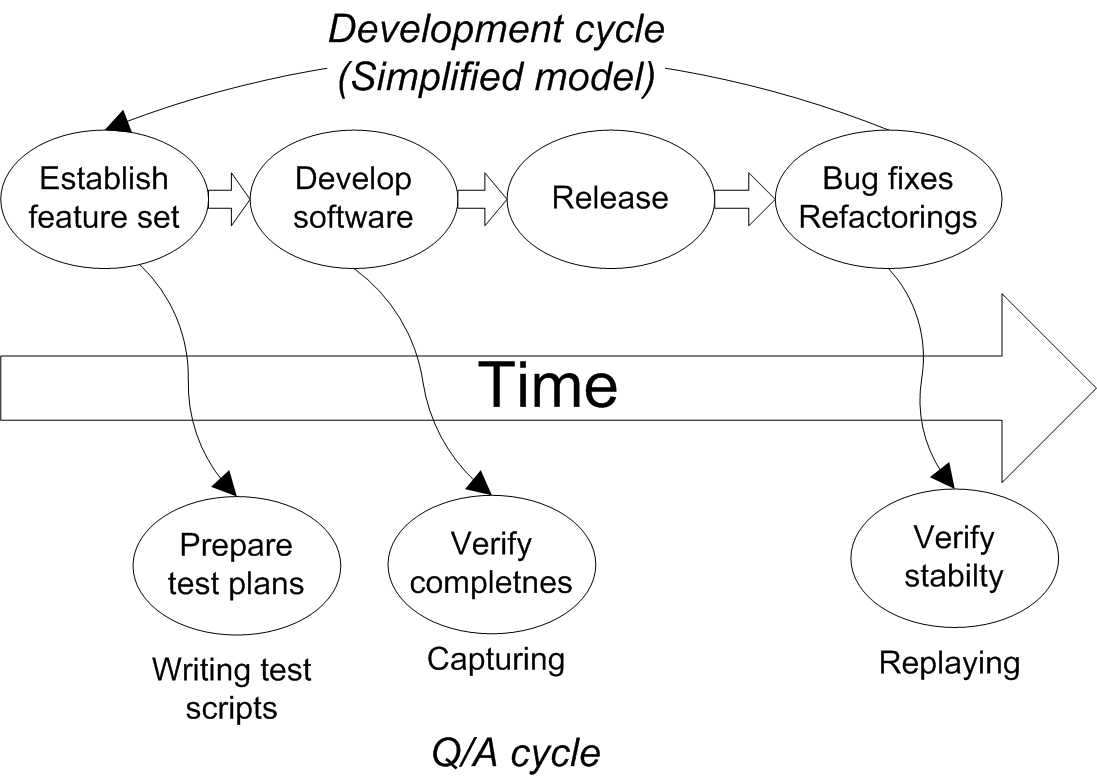
\includegraphics[width=.9\linewidth]{figures/process-outline-2}
\end{center}
\caption{Capture-replay regression test scenario in parallel to software development life cycle.}%
\label{fig:process-outline-2}
\end{figure}

In this thesis we would like to focus on the difficulties of testing mobile applications and possibilities of
automation of this process.  


\subsection{Problems of GUI Testing}

Testing mobile applications is different compared to desktop software because of several
reasons:

\begin{itemize}
    \item mobile software is written on an emulator and eventually runs on the actual device,

    \item there are less or more subtle differences between emulators and devices (and in particular across devices from different
    vendors) in terms of supported APIs, hardware and Java Virtual Machine implementation details,
    
    \item uploading and testing the application on each and every device is a tedious, time-consuming process,
    
    \item the final release of the software often differs from the development version due to obfuscation, macro expansion
    and other code-manipulation techniques.
\end{itemize}

Both programming and particularly testing are much more difficult in such an environment
compared to writing programs for the desktop. Each mobile phone, for example, has a different
hardware configuration: display size and capabilities (number of colors), size of memory and varying
computational power. Application interfaces defined by the J2ME specification and considered a
`standard', are implemented by different vendors and often contain differences that must be taken
into account, increasing the complexity of the program. The same application looks, but often also
\emph{behaves} a bit different depending on the target device it was installed on. 
The key differences between mobile and traditional software development was summarized in 
Table~\ref{tab:environments}.


\begin{table}[t]%
\caption{Differences between development and testing of mobile and traditional (desktop and server) applications.}%
\label{tab:environments}
\scriptsize
\begin{tabularx}{\linewidth}{>{\raggedright}p{2cm} @{\hspace{3mm}} >{\rightskip\fill}X @{\hspace{3mm}} >{\rightskip\fill}X}
\toprule
\tabcaption{Element} & \tabcaption{Mobile} & \tabcaption{Traditional} \\ \midrule

Test recording
    &
    Lack of programmatic access to recording GUI events.
    Emulation of user interaction impossible.
    &
    Standard \texttt{java.awt.Robot} class
    for re\-cor\-ding GUI events. \\ \addlinespace[1mm]

Deployment automation
    &
    Tedious (manual) routine of on-device deployment and
    testing.
    & 
    Deployment usually fully automatic. Testing and harvesting
    test results automatic and relatively easy. 
    \\ \addlinespace[1mm]

Test environment differences
    &
    Differences across devices (different virtual machines, varying memory and resource availability).
    Requirement to run tests on all possible configurations.
    &
    Virtually identical development and deployment/ testing
    environment. In very rare cases operating-system specific. \\ \addlinespace[1mm]

Programming interfaces 
    &
    A number of non-standard APIs and proprietary
    solutions (playing sounds, access to external ports, access to 
    the current display). 
    &
    More mature and standard APIs, portable across JVMs
    from different vendors. \\

\bottomrule
\end{tabularx}
\end{table}


Because of the differences in hardware and software, software for mobile devices should be tested on
each individual piece of equipment separately. Knowing that the deployment process takes some time,
testing quickly becomes a tedious routine software developers grow to hate in no time. 

The GUI applications in particular resist rigorous testing.
A common solution is to \emph{record} real scenarios of user interaction with the program (directly
off the application's screen) and then try to reproduce the same stimuli at the testing phase,
validating program's response accordingly. This kind of procedure is made possible with various
GUI automation tools and programming interfaces; programs for recording GUI
events are called \emph{robots} and the technique is dubbed \emph{capture-replay testing methodology}.

Writing a \emph{capture-once}, \emph{replay-on-all} testing framework seems like a natural answer addressing
the problem, even if the experiences with this type of tests in desktop applications are not always
positive (contrary to the desktop, mobile applications are much simpler, so test scenarios
should retain manageable size). 
Unfortunately, the J2ME environment does not offer any system-level 
support with respect to handling GUI events and any other events for that matter. 
We replace this required and missing functionality with
an automatic preprocessing of the binary code of the tested program (a process generally
known as \emph{bytecode-level instrumentation} or \emph{code injection}).
The testing framework we then build upon this idea -- called RobotME -- is designed to support automated recording
of the interaction with a mobile application, regardless of the aspects of implementation. This way a test script recorded
once (during development, on an emulated device, for example) can and should run identically on other devices. 
The test validation phase can be executed both on real devices and emulators of mobile devices, effectively making the testing
shorter, easier and repeatable.


\section{Motivation and Goals}

Java 2 Micro Edition environment (J2ME) lacks most of the above facilities for implementing GUI
automation. All existing products (research or commercial) for testing mobile applications in J2ME
are very simple and lack capture-replay testing support. This fact raises the following questions:
%
\begin{itemize}
    \item In spite of technical difficulties, is it possible to devise a cross-platform architecture 
	facilitating unit and integration testing of mobile applications? How much overhead (code, time) 
	is required for running such a solution?
    \item Is there an industry need for integration tests aimed for mobile applications?
    \item How much time and resources can we save by implementing semi- or fully automatic
    integration tests in J2ME?
\end{itemize}
%
The first question is very technical in nature, but poses great technical difficulties because
of the limited functionality available in the J2ME environment. We believe overcoming such major
obstacles, although definitely with a technical in nature, qualifies as a research activity. In this thesis we
would like to design and implement an architecture that allows capture and replay of GUI events in the J2ME environment
by means of dynamic code injection. This would constitute a significant improvement over all the products available 
in the literature and on the market.

As for the last question, there seems to be no direct answer to how using regression tests
translates into economic value. While we could try a controlled user-study to assess the time or effort 
savings gained from using regression tests, this kind of experiment is always subjective 
and lacks the real-life constraints of a commercial company's environment. This problem is 
actually omnipresent with respect to software testing in general -- common sense suggests tests provide 
certain measurable value, but hard estimation of this value is very difficult.

Having these issues in mind we set the following goals for this thesis:
\begin{itemize}
    \item find a portable, efficient technical solution for implementing capture/replay tests under 
    J2ME environment,
    \item implement this solution and show its feasibility on a range of popular 
    mobile phones and emulators.
\end{itemize}


\section{Thesis Outline}

In Chapter 2 we present theoretical background to software testing in general and
to GUI and mobile application testing in particular. We also describe some of existing
solutions that attempt to solve the problem of mobile applications testing. Chapter 3 introduces
high-level design and architecture of the RobotME framework. We then subsequently follow with some 
limited details of implementation, required to understand the proposed solution in Chapter 4.
Chapter 5 contains the results of performed experiments. We present a summary and conclusions from
the presented work in Chapter 6.
